\section{Data}
\label{sec:data}

\subsection{Source}

All data come from the CPCB \emph{Surface Water Quality (Manual)} datasets published on the National Water Data Portal (\texttt{nwdp.nwic.gov.in}). The portal splits the NWMP record into three thematic tables, each further split by state/UT and time bucket:

\begin{table}[h]
\centering\small
\caption{Raw downloads. The ``1961--2020'' file bucket is a portal label only: every record actually falls between 2018-01-01 and 2024-07-01.}
\label{tab:raw}
\begin{tabular}{lrrrl}
\toprule
Table & Files & Rows & Size & Parameters used here \\
\midrule
Physical   & 70 & 94,159  & 15 MB & EC, Turbidity \\
Chemical   & 71 & 109,683 & 27 MB & pH, DO, Nitrate-N \\
Biological & 70 & 107,537 & 16 MB & BOD, Fecal coliform, Total coliform \\
\midrule
Total      & 211 & -- & 57 MB & 8 parameters \\
\bottomrule
\end{tabular}
\end{table}

\subsection{Cleaning and integration pipeline}

The pipeline (\texttt{scripts/build\_dataset.py}, summarised in \cref{fig:pipeline}) performs the following steps.

\begin{enumerate}
  \item \textbf{Parse and de-duplicate.} Acquisition timestamps are parsed to dates. Same-station, same-day repeat readings within a file are averaged.
  \item \textbf{Join.} The three tables are \emph{not} row-aligned after 2020: physical parameters are logged far less often than chemical and biological ones. They are therefore outer-joined on (station, state, district, latitude, longitude, date) rather than concatenated by position.
  \item \textbf{River filter.} The structured \texttt{River} field is populated for only 0.08\% of rows. River stations are therefore identified by matching about 95 Indian river names against the free-text station name. Stations whose names contain groundwater keywords (borewell, hand pump, tube well, piezometer, \dots) are excluded, since early versions matched, for example, a borewell named after a person called Krishna.
  \item \textbf{Plausibility flags.} Physically impossible readings (e.g.\ pH 78.2, EC of 25 million \si{\micro S/cm}) are flagged per parameter rather than silently altered. The 3 affected river rows are excluded from the ground truth.
\end{enumerate}

A systematic audit of this pipeline found and fixed two real defects (a second groundwater false positive and the missing plausibility flags). It also cleared one suspected defect: 14 stations with two coordinate pairs turned out to be genuinely distinct nearby sampling points. The result is a river table of \textbf{32,968 usable visits at 888 stations on 87 rivers}. Re-running the pipeline on a fresh environment for this report reproduced all three processed files byte-for-byte.

\begin{figure}[t]
  \centering
  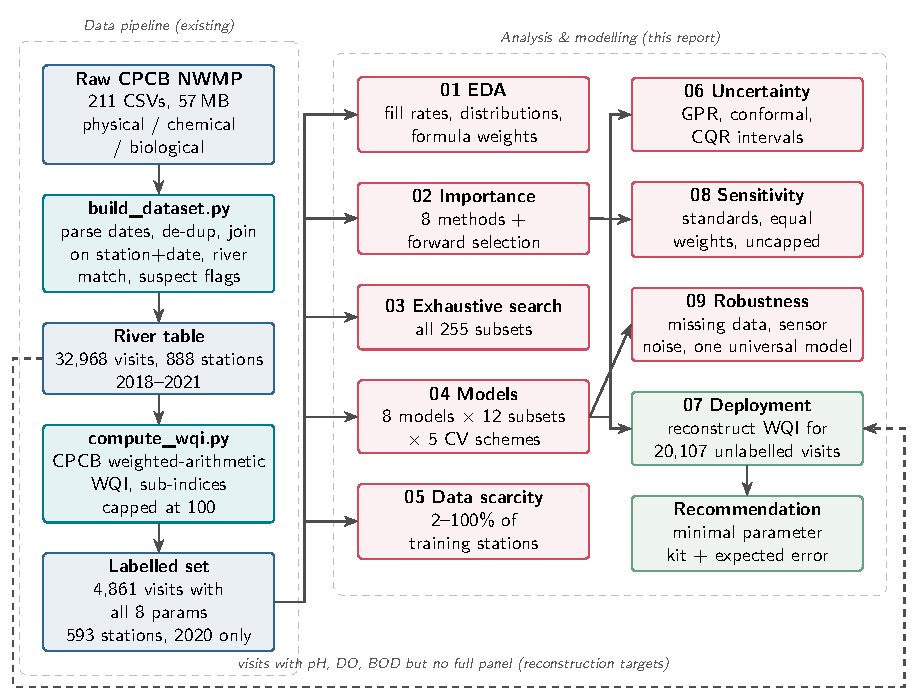
\includegraphics[width=0.92\textwidth]{pipeline.pdf}
  \caption{End-to-end pipeline. Blue/teal: the data pipeline that produces the labelled set. Red: the analyses reported here (script numbers in \texttt{scripts/}). Green: deployment on visits that lack a full panel.}
  \label{fig:pipeline}
\end{figure}

\subsection{Parameter availability: the full panel exists for one year only}
\label{sec:data-availability}

\Cref{fig:fill} shows, per year, the fraction of river visits that report each of the eight usable parameters. Temperature, COD, TDS, total solids, colour and odour were excluded earlier because each is recorded in under about 6\% of rows.

\begin{figure}[t]
  \centering
  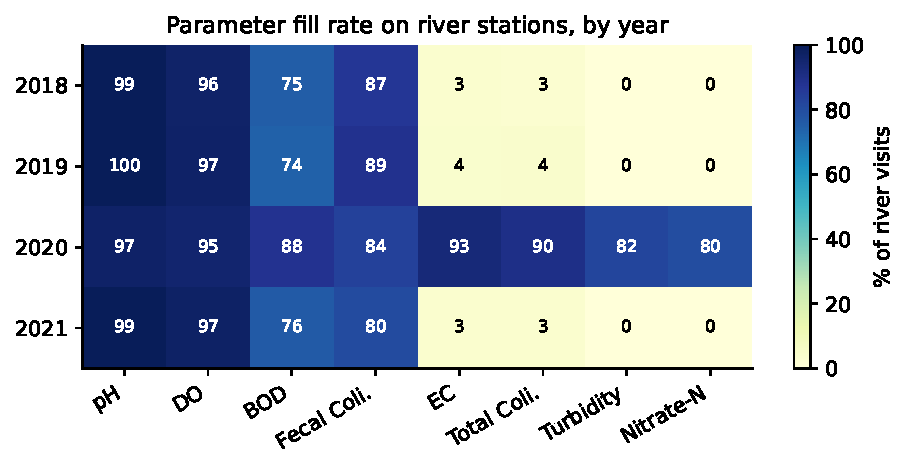
\includegraphics[width=0.85\textwidth]{fig_eda_fill_by_year.pdf}
  \caption{Fill rate (\% of river visits reporting the parameter) by year. pH, DO, BOD and fecal coliform are reported routinely every year. EC, total coliform, turbidity and nitrate-N were reported almost exclusively in 2020.}
  \label{fig:fill}
\end{figure}

This is the single most consequential property of the data and was not visible in earlier, pooled fill-rate summaries. pH, DO, BOD and fecal coliform form a \emph{routine panel}, reported on 74--99\% of visits in every year. EC, total coliform, turbidity and nitrate-N were reported on 80--93\% of visits in 2020 but on 0--4\% in 2018, 2019 and 2021. Three consequences follow:

\begin{itemize}
  \item The ground-truth WQI can be computed only for 2020 visits. A ``train on early years, test on later years'' split is impossible, so temporal generalisation is examined through a held-out-season scheme instead (\cref{sec:methods-cv}).
  \item Outside 2020, the subsets \sub{S5} and \sub{S7} originally proposed in the project methodology are not actually available at river stations, because EC, total coliform and turbidity are missing there. The routine panel \sub{S4-routine} (pH, DO, BOD, fecal coliform) and its core \sub{S3} (pH, DO, BOD) are what reduced-parameter monitoring looks like in practice.
  \item The 2018, 2019 and 2021 visits are a natural, real (not simulated) data-scarce deployment target (\cref{sec:res-deploy}).
\end{itemize}

The resulting gap is large\optref{fig:funnel}. Of 32,968 visits, 24,993 (75.8\%) report \sub{S3} and 21,547 (65.4\%) the routine four-parameter panel, but only 4,861 (14.7\%) report all eight parameters.

\iffull
\begin{figure}[t]
  \centering
  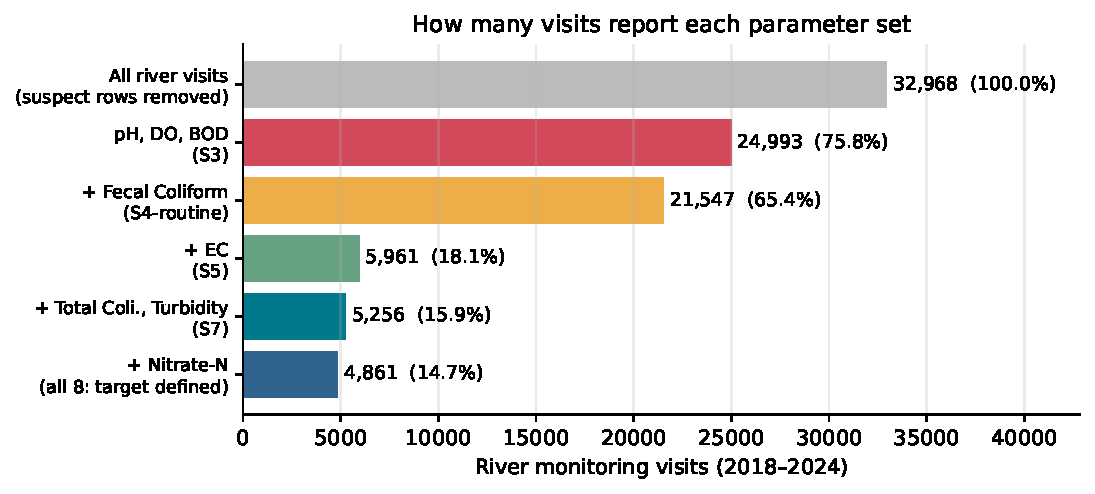
\includegraphics[width=0.85\textwidth]{fig_eda_funnel.pdf}
  \caption{Availability funnel: number of river visits that report each nested parameter set. Only the last bar carries a computable ground-truth index.}
  \label{fig:funnel}
\end{figure}
\fi

\subsection{The labelled set}

The 4,861 fully-observed visits come from \textbf{593 stations on 58 rivers in 21 states}, all in 2020. A station contributes between 1 and 19 visits (median 9). Coverage spans the Himalayan rivers of Himachal Pradesh and Punjab, the Ganga main stem (909 visits), the Deccan rivers (Godavari, Krishna, Cauvery, Tungabhadra) and the central/western rivers (Narmada, Tapi, Mahi, Chambal) (\cref{fig:map}). Monsoon months (June--September) contribute 1,819 visits, post-monsoon 1,118, pre-monsoon 1,026 and winter 898.

\begin{figure}[t]
  \centering
  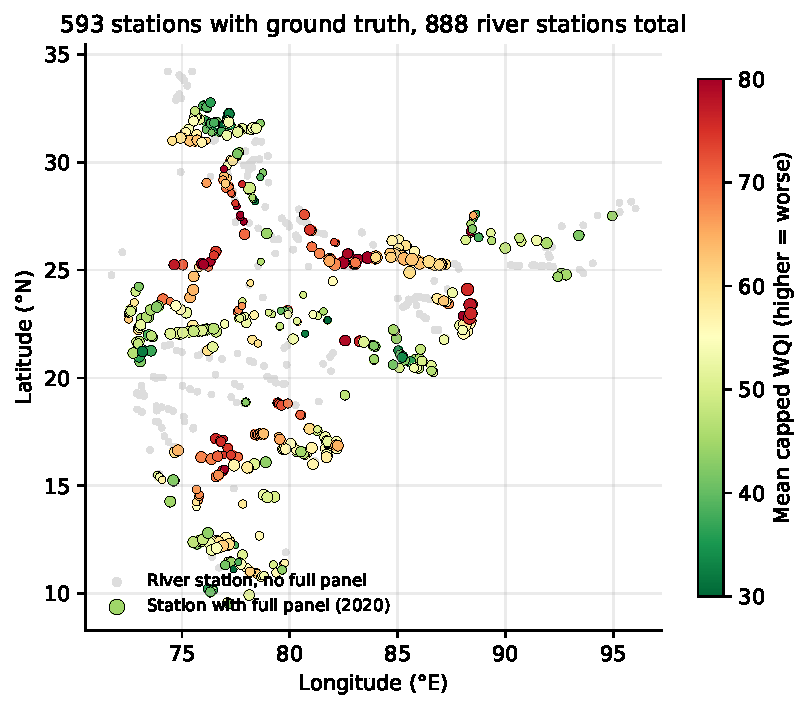
\includegraphics[width=0.62\textwidth]{fig_eda_station_map.pdf}
  \caption{River stations. Coloured: the 593 stations with full-panel ground truth, coloured by mean capped WQI and sized by number of visits. Grey: river stations without a full panel.}
  \label{fig:map}
\end{figure}

\Cref{tab:describe} summarises the eight parameters. Six of them are extremely right-skewed (skewness 8--35): turbidity ranges up to 3,640 NTU during monsoon silt events, and BOD up to 294 mg/L below a sewage inflow on the Ganga. \iffull\Cref{fig:paramdist} shows the distributions against each parameter's standard. \fi Turbidity exceeds its 10 NTU standard on 47.6\% of visits, fecal coliform its 500 MPN/100\,mL standard on 33.7\%, and BOD its 3 mg/L standard on 12.2\%.

\begin{table}[t]
\centering\small
\caption{Parameter statistics in the labelled set ($n=4{,}861$).}
\label{tab:describe}
\begin{tabular}{lllrrrrrr}
\toprule
Parameter & Unit & Measurement & Median & 5\% & 95\% & Max & Skew & \% $>S_i$ \\
\midrule
pH & -- & probe, instant & 7.80 & 7.00 & 8.49 & 8.9 & $-0.4$ & 2.9 \\
DO & mg/L & probe, instant & 7.20 & 4.10 & 9.30 & 13.0 & $-1.1$ & 7.9 \\
BOD & mg/L & lab, 5 days & 1.70 & 0.20 & 5.00 & 294 & 35.4 & 12.2 \\
Turbidity & NTU & probe, instant & 9.00 & 0.92 & 236 & 3,640 & 9.5 & 47.6 \\
Nitrate-N & mg N/L & kit / lab & 0.50 & 0.06 & 2.70 & 98 & 19.5 & 0.9 \\
Fecal coliform & MPN/100mL & lab, 24--48 h & 130 & 1 & 90,000 & 840,000 & 8.2 & 33.7 \\
EC & \si{\micro S/cm} & probe, instant & 323 & 91 & 1,943 & 61,120 & 8.6 & 10.9 \\
Total coliform & MPN/100mL & lab, 24--48 h & 540 & 32 & 160,000 & 2,400,000 & 12.4 & 22.1 \\
\bottomrule
\end{tabular}
\end{table}

\iffull
\begin{figure}[t]
  \centering
  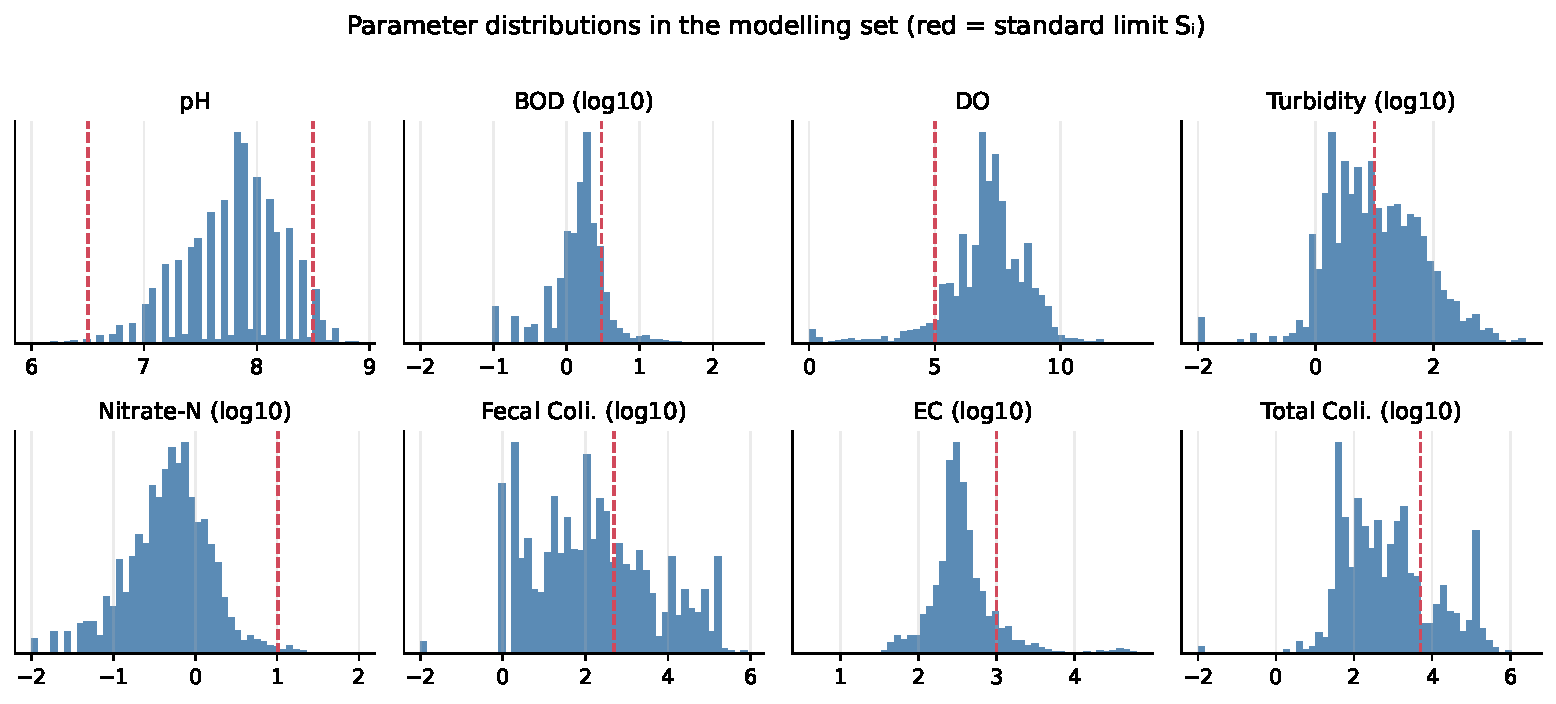
\includegraphics[width=\textwidth]{fig_eda_param_distributions.pdf}
  \caption{Parameter distributions in the labelled set. Skewed parameters are shown on a $\log_{10}$ axis. Dashed red lines mark the standard $S_i$ (for pH, the 6.5--8.5 band).}
  \label{fig:paramdist}
\end{figure}
\fi
